\documentclass{article}
\usepackage[utf8]{inputenc}
\usepackage{graphicx}
\graphicspath{ {images/} } 
\begin{document}
\title{Application of Graph Colouring}
\author{Shashvat Kedia(1610110347) , Raghav Kirpekar(1610110271) ,  Raman Dutt(1610110357)}
\maketitle
\begin{abstract}
A Graph G is a mathematical structure of consisting of two sets V(G) (vertices of G) and E(G) (edges of G). Proper colouring of a graph is an assignment of colours to the vertices such that the adjacent vertices are coloured differently.
This paper discusses colouring on graphs with \textit{Mathematica} and \textit{WebMathematica}. \hfill \break
We draw any graph and also try to show weather it has a Eulerian and Hamiltonian cycles.
\end{abstract}
\section{Introduction}
Graph theory would not be what it is today if there had been no colouring problems. A Graph G is a mathematical structure of consisting of two sets V(G) (vertices of G) and E(G) (edges of G).\hfill \break
Vertex colouring is a hard combinatorial optimisation problem we apply several operations on graphs to give different graphs. in addition, we colour vertices to these obtained graphs properly. Many of these graphs are truly beautiful and they provide a wide range of structures to manipulate and study.\hfill \break
A complete graph is a simple graph such that every pair of vertices is joined by an edge. Some number of vertices connected in a close chain is called a cycle. A graph which is obtained by joining a new vertex to every vertices of a cycle is called a Wheel. A connected Acyclic graph is called a tree \cite{1}. \hfill \break
\textbf{Graph Colouring Algorithms} : There are many sequential techniques for colouring a graph. One of them is Greedy Graph Colouring. Greedy Colouring concentrates on carefully picking the next vertex to colour and the colour for the next vertex. There are two basic ordering techniques used First Fit and Degree Based Ordering.\hfill \break
\textbf{First Fit} : The First Fit colouring algorithm is given the set of vertices in an arbitrary order and the job of the algorithm is to assign lowest legal colour to each vertex. First fit is an O(n) time algorithm. \hfill \break
\textbf{Degree Based Ordering} : Degree Based Ordering is considered a better strategy as compared to First Fit because it uses a certain criterion for choosing the vertex to be coloured from a set of uncoloured vertices rather than picking the next vertex from an arbitrary order. Some of the well known Degree based Ordering techniques are Largest Degree Based Ordering and Saturation Degree Based Ordering.\hfill \break
\textbf{Largest Degree Based Ordering} : Ordering the vertices by decreasing degree proposed by C. Avanthay, A. Hertz, N. Zufferey \cite{5}. it is considered one of the oldest ordering strategies.Suppose the vertices v1, v2…,vi-1 have been chosen and coloured. Vertex vi is chosen to be the vertex with the maximum degree among the set of uncoloured vertices. Largest Degree Ordering provides a better colouring that First Fit since during each iteration  chooses a vertex with the highest number of neighbours which potentially produces he highest colour. Largest Degree Based Ordering Algorithms has a complexity of O($n^{2}$). 
\textbf{Saturation Degree Based Ordering} :  Saturated degree ordering was proposed by E.Falkenauer \cite{6}. The saturation degree of a vertex is defined as the number of differently coloured vertices the vertex is adjacent to.  Saturation Degree Based Ordering works as follows :  Suppose that vertices v1, v2,…,vi-1 have been chosen and colored. Then at step i, vertex vi with the maximum Saturation degree is selected. While choosing a vertex of maximum saturation degree, ties are broken in favor of the vertex with the largest degree. \hfill \break
Saturation Degree Based Ordering provides better colouring as compared Largest Degree Based Ordering since it first colours the vertices most constrained by previous colour choices. Saturation Degree Based Ordering algorithm has a complexity of O($n^{2}$).

\section{Graph Colouring with WebMathematica}
\textit{WebMathematica} is a technology developed by Wolfram research which enables instructors to create websites that allow users to compute and visualize results directly from a web browser. It is based on a standard Java technology called servlets. It allows a site to deliver HTML(Hyper Text Markup Language) pages that are enhanced by the addition of Mathematica commands \cite{2}. When a request is made for one these pages, the commands are evaluated and the computed result is placed in the page. \hfill \break In this section we give applications to colour the vertices of the graphs with \textit{WebMathematica}.

\subsection{Vertex Colouring}
The most applications involving vertex colouring are concerned with finding the minimum number of colours required so that two adjacent vertices cannot have the same colour. A proper vertex colouring of a Graph is an assignment from its vertex set to a coloured set that any two adjacent vertices are assigned two different colours. \hfill \break
The chromatic colour of a Graph G denoted by \(\chi\)(G), is the minimum number of different colours required for a proper vertex colouring of G. \hfill \break Applications of vertex colouring include timetable scheduling, assignment of radio frequencies and computer optimization. We use commands in the Combinatorica package with Mathematica to colour the vertices of the graph given below\cite{3}. \hfill \break
\hfill \break
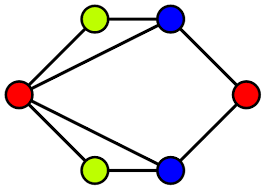
\includegraphics{vertexcolouring}.
\hfill \break

\subsection{Edge Colouring}
Edge colouring is an optimization problem: An edge colouring of a graph G is an assignment of colours to the edges of G such that edges with a common endpoint have different colours. The problem to colour edges is an NP problem which means that the algorithm used for the solving th problem does not have a polynomial time complexity.\hfill \break
Commands in Mathematica can be used to colour edges of graphs and give web-based examples with \textit{WebMathematica}\cite{3}.\hfill \break
\hfill \break
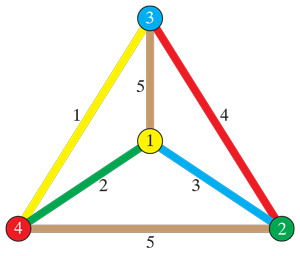
\includegraphics{edgescolouring}. \hfill \break
\hfill \break
If the user presses the Wheel button nd enter the number of vertices, he/she can get the dge-coloured graph.

\section{Generating Graphs with  WebMathematica}
Some of the most important operations on Graphs are sum,union, join and product of two graphs etc. These operations can be performed on common graphs, complete graphs, cycle, wheel and random tree using \emph{\textit{Web Mathematica}}. \hfill \break
\textbf{Join of two graphs} : The union of two graphs with addition f edges between all pairs of vertices from different graphs is know as the join of two graphs. \hfill \break
 \textbf{Union of two graphs} : The union of two graphs is formed by taking the union of the vertices and edges of the graphs. Thus the unions of graphs is always disconnected. \hfill \break
 \textbf{Sum of two graphs} : The sum operation of two graphs is to take the edges of the second graph and add them to the first graph. \hfill \break
 \textbf{Product of two graphs} : The product of two graphs G\( \times \)H has a vertex set defined by he Cartesian product of the vertex sets of G and H
 There is an edge between (u,v) and (s,t) if u = s and v is adjacent to t in H or
  v = t and u is adjacent to s in G. \hfill \break
 
 \section{Cycle Structure in Graphs with  \hfill \break WebMathematica}
 A Cycle in a graph is a simple closed path. We will represent a cycle in Graph G as a list of vertices C = v1,v2,........,v1 such that there is an edge of G from each vertex to the next in G.
 
 \subsection{Eulerian Cycle}
 An Eulerian Cycle, also called a Eulerian Circuit is a path with starts and ends at the same vertex in graph G. In other words it is a graph cycle which uses each vertex edge exactly once. \hfill \break
 Euler initiated the study of Graph theory in 1736 with the famour seven bridges of Konigsberg Problem the town of Konigsberg straddled the Pregel river with a total of seven bridges connecting the two shores and two islands.
 The tows folk were interested in crossing every bridge exactly once and returning to the starting point. \hfill \break
 An Eulerian cycle is a complete tour of all the edges of a graph. The term circuit is often used instead of cycle since each vertex can be visited more then once. \hfill \break
 We use \textit{WebMathematica} to find the Eulerian cycle and to give web based examples. If the number of the vertices is entered, it is possible to see the Eulerian cycle in that graph if there exists one \cite{4}. \hfill \break
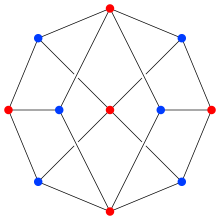
\includegraphics{euleriancyclegraphs}
 \hfill \break
 
 \subsection{Hamiltonian Cycle}
 Hamiltonian Cycle of a Graph G is a cycle which visits each vertex in G exactly once, as opposed to a Eulerian Cycle which visits each edge exactly once. A Hamiltonian Path is a path between two vertices of a graph that visits each vertex exactly once. The problem of computing a Hamiltonian Cycle is fundamentally different from the problem of computing a Eulerian Cycle because testing whether a graph is Hamiltonian is NP complete which means that the algorithm used for computing weather a graph contain a Hamiltonian circuit does not have a polynomial time complexity. \hfill \break
 We use \textit{WebMathematica} to find the Hamiltonian cycle and to give web based examples. If the number of the vertices is entered it is possible to see the Hamiltonian cycle in that graph if there exists one\cite{4}. \hfill \break
 \hfill \break
 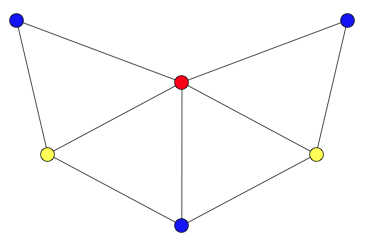
\includegraphics{hamiltoniancyclegraphs}
 \hfill \break

\subsection{An Application}
Some scheduling problems can induce a graph colouring i.e An assignment of colours to vertices of a graph. We discuss a simple example for colouring the vertices of a graph with a small number k of colours and present computational results for calculating the chromatic number i.e the minimum possible value of such a k. \hfill \break
\textbf{Example} : Set of students: S1, S2, S3, S4, S5, S6, S7, S8, S9 Examination subjects
for each group: {algebra, real analysis, and topology}, {algebra, operations
research, and complex analysis}, {real analysis, functional analysis, and
topology}, {algebra, graph theory, and combinatorics}, {combinatorics, topology,
and functional analysis}, {operations research, graph theory, and coding
theory}, {operations research, graph theory, and number theory}, {algebra,
number theory, and coding theory}, {algebra, operations research, and real
analysis}. \hfill \break
Let S be a set of students, P = \(\{1, 2, 3, 4, 5, 6, 7, 8, 9, 10\}\) be the set of
examinations respectively algebra,real analysis, topology, operational research,
complex analysis, functional analysis, graph theory, combinatorics, coding
theory, and number theory. S(p) be the set of students who will take the
examination p \(\in\) P. Form a graph G = G(P, E), where a, b \(\in\) P are adjacent if and only if S(a) \( \bigcap\) S(b) \(\neq\)  \(\Phi\). Then each proper vertex colouring of G yields an examination schedule with the vertices in any color class representing the
schedule on a particular day. Thus \(\chi\)(G) gives the minimum number of days required for the examination schedule.  \hfill \break
 5 days are required and you can see below the lessons in the same parenthesis which are on the same day
\(\{\{1, 6\}, \{2, 8, 9\}, \{3, 4\}, \{5, 7\}, \{10\}\}\)

  \begin{thebibliography} {1}
\bibitem {1} Jonathan,G and Jay,Y : Graph theory and its application, CRC Press, (1999).

\bibitem {2} Pemmaraju,S. and Skiena,S. : Computational Discrete Mathematics, Cambridge University Press,(2003).

\bibitem {3} Ufuktepe,U. Bacak,G. and Beseri,T. : Graph colouring with \textit{WebMathematica}, Springer-Verlag,(2003).

\bibitem{4} Google Images

\bibitem{5} C. Avanthay, A. Hertz, N. Zufferey, A variable neighborhood search for graph coloring, European Journal of Operational Research 151 (2) (2003) 379–388. 

\bibitem {6} E. Falkenauer, A hybrid grouping genetic algorithm for bin packing, Journal of Heuristics 2 (1) (1996) 5–30.

\bibitem {7}  

\end{thebibliography}

\end{document}